\documentclass[14pt]{beamer}
\usetheme{PaloAlto}
\usecolortheme{seahorse}
\usepackage[T1]{fontenc}
\usepackage[utf8]{inputenc}
\usepackage{lmodern}
\usepackage{listings}
\usepackage{tikz}
\usetikzlibrary{circuits.ee.IEC}
\usepackage{placeins}
\usepackage{standalone}
\usepackage{dirtree}
\setbeamertemplate{footline}[frame number]

\lstset{
basicstyle=\ttfamily\tiny,
breaklines=true,
postbreak=\raisebox{0ex}[0ex][0ex]{\ensuremath{\color{red}\hookrightarrow\space}}}


\title{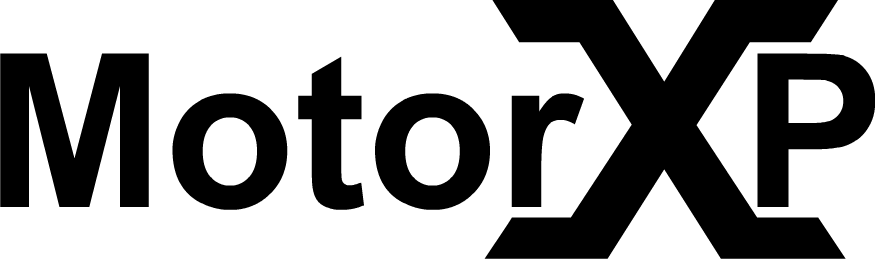
\includegraphics[height=1cm]{../images/MotorXP}}
\author{Christian Brunner, Andreas Kölbl, Ricardo Krause, Bernd Krupinski, Andreas Lackner, Michael Schleinkofer, Franz Welker}

\begin{document}
\begingroup
\makeatletter
\setlength{\hoffset}{-.5\beamer@sidebarwidth}
\makeatother
\begin{frame}[plain]
  \titlepage
\end{frame}
\endgroup
  \title{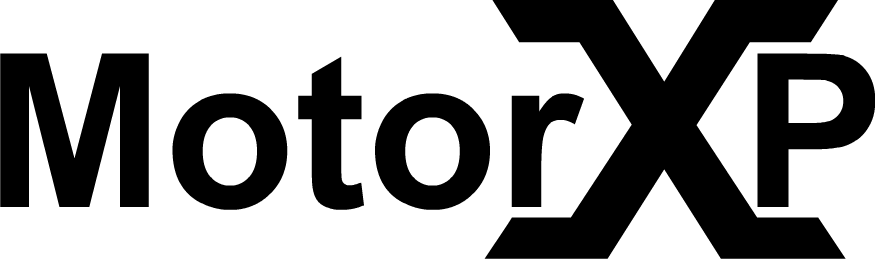
\includegraphics[height=0.5cm]{../images/MotorXP}}
  \author{}

\begin{frame}{MotprXP}
\begin{itemize}
	\item BLDC-Motor
	\item Sensorik
	\item Ansteuerung
	\item Kommunikation
	\item Regelung
	\item Visualisierung
	\item Test und Analyse
	\item Simulation
\end{itemize}
\end{frame}


\section{Projekt Start}
\begin{frame}{Projekt Start}{Projekt Start Phase}
  \begin{itemize}
    \item Projekt Auftrag
    \item Projekt Plan
    \item Versionsverwaltung
    \item Kommunikation
    \item Dokumentenmanagement
  \end{itemize}
\end{frame}

\begin{frame}{Projekt Start}{Projekt Auftrag}
\begin{figure} [htbp]
 \centering
 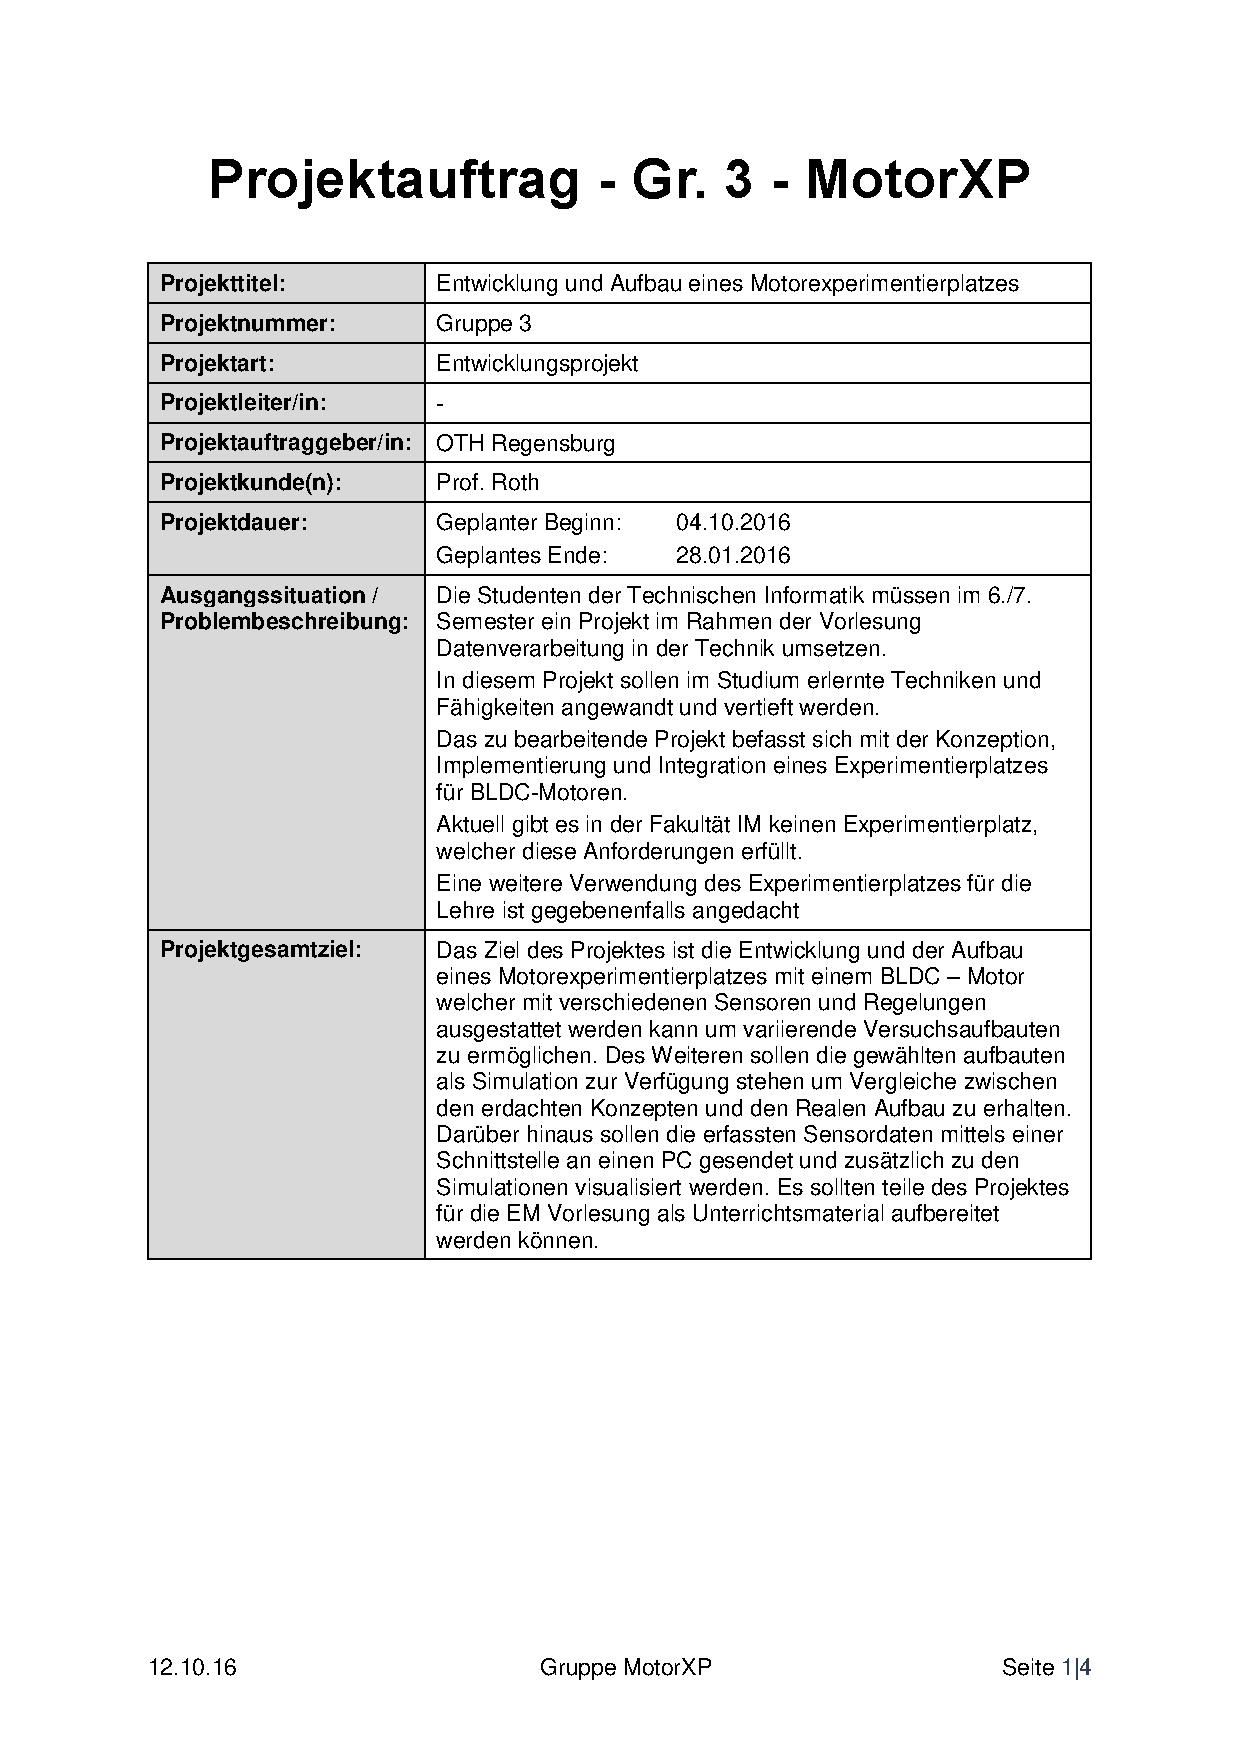
\includegraphics[scale=0.3]{../projectdefinition/Appendix/Projektauftrag_Gruppe3_MotorXP.pdf}
\end{figure}
 \end{frame}
 \begin{frame}{Projekt Start}{Projekt Auftrag}
\begin{figure} [htbp]
 \centering
 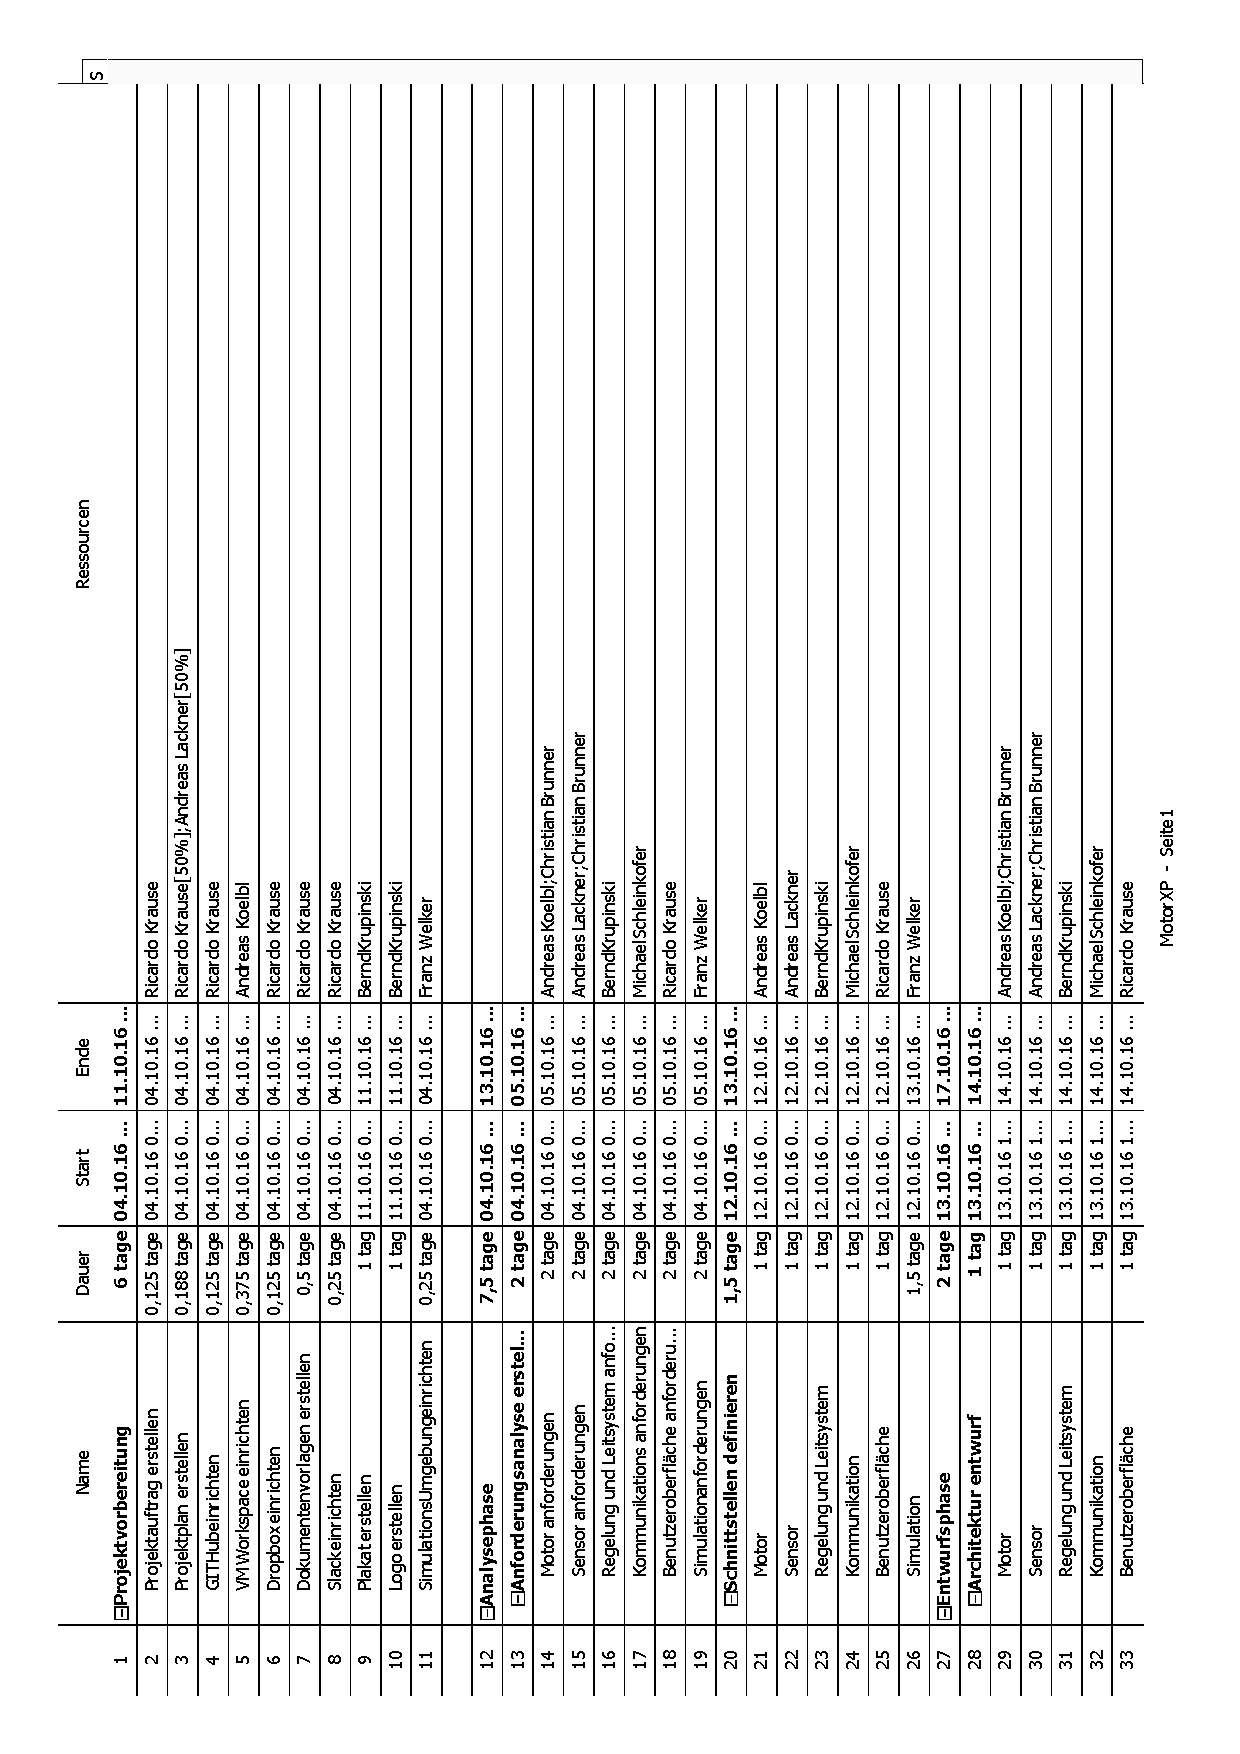
\includegraphics[scale=0.3,angle=270]{../projectdefinition/Appendix/DT_Projektplan_Gr3_MotorXP_2.pdf}
\end{figure}
 \end{frame}
  \begin{frame}{Projekt Start}{Github}
\begin{figure} [htbp]
 \centering
 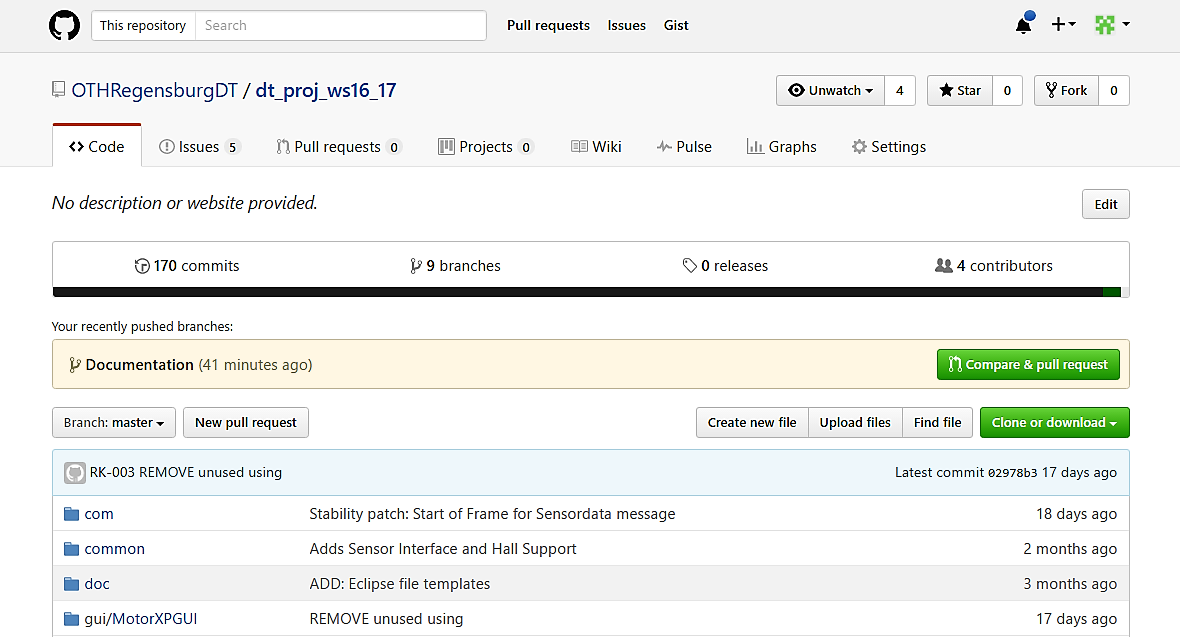
\includegraphics[scale=0.3]{../projectdefinition/Bilder/Github.png}
\end{figure}
 \end{frame}
  \begin{frame}{Projekt Start}{Slack}
\begin{figure} [htbp]
 \centering
 \includegraphics[scale=0.35]{../projectdefinition/Bilder/Slack.png}
\end{figure}
 \end{frame}
   \begin{frame}{Projekt Start}{Dropbox}
\begin{figure} [htbp]
 \centering
 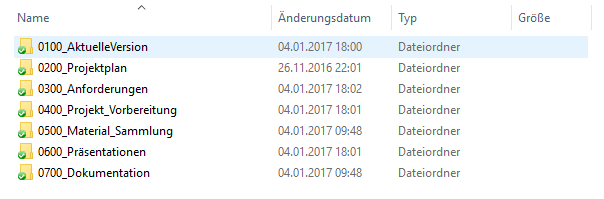
\includegraphics[scale=0.5]{../projectdefinition/Bilder/FolderStructure.png}
\end{figure}
 \end{frame}

\section{Sensorik}
\subsection{Anforderungen}

\begin{frame}{Sensorik}{Anforderungen}
  \begin{itemize}
    \item Welche Daten brauchen wir?
    \begin{itemize}
    \item Kommutierungszeitpunkt
    \item Umdrehungsgeschwindigkeit
    \item Drehwinkel
    \item Temperatur
    \end{itemize}
    \item Welche Sensoren stehen zur Verfügung?
    \begin{itemize}
      \item Drei Hall-Sensoren
      \item Inkrementalgeber
      \item NTC Temperatursensor
    \end{itemize}
  \end{itemize}
\end{frame}


\subsection{Sensor Interface}

\begin{frame}{Sensorik}{Sensor Interface}	
  \begin{itemize}
    \item Kapselung in ein eigenes Softwaremodul
    \item Zugriff auf Sensorwerte über ein definiertes Interface
    \begin{itemize}
      \item Geringer Integrationsaufwand
      \item Gute Portierbarkeit
    \end{itemize}
  \end{itemize}
  \dirtree{%
  .1 Sensor.h.
  .2 Sensor\_Hall.h.
  .2 Sensor\_QuadratureDecoder.h.
  .2 Sensor\_Temperature.h.
  }  
\end{frame}

\begin{frame}{Sensorik}{Sensor Interface}	
 \begin{figure} [htbp]
  \centering
  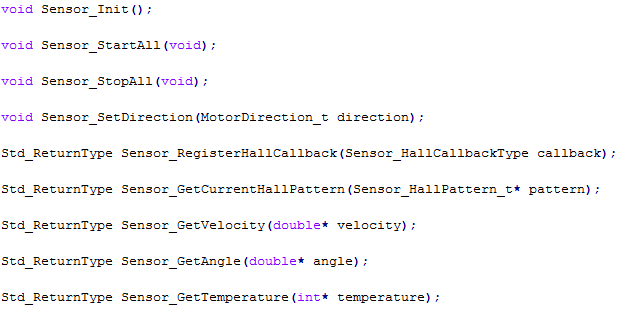
\includegraphics[scale=0.6]{Sensor/sensor_interface.PNG}
 \end{figure}
\end{frame}


\subsection{Hall-Sensoren}

\begin{frame}{Sensorik}{Hall-Sensoren}	
 Digitale Hall-Sensoren zur Messung von Magnetfeldern
 \begin{figure} [htbp]
  \centering
  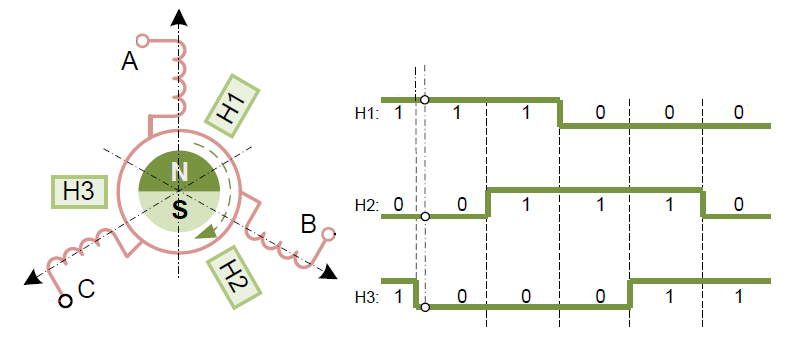
\includegraphics[scale=0.4]{Sensor/hall_sample.PNG}
 \end{figure}
\end{frame}

\begin{frame}{Sensorik}{Hall-Sensoren}	
 \begin{itemize}
 \item Messung des Hall-Patterns mit POSIF
 \item Zwei mögliche Events
	 \begin{itemize}
	 \item Correct-Hall-Event
	 \item Wrong-Hall-Event
	 \end{itemize}
 \item Ermittlung des motorspezifischen Hall-Patterns
 \end{itemize}
 \begin{figure} [htbp]
   \centering
   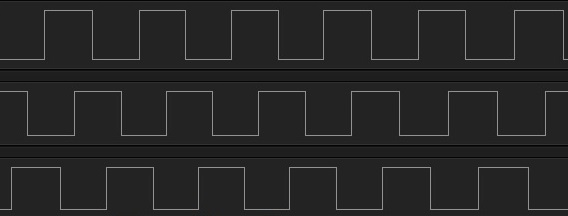
\includegraphics[scale=0.3]{Sensor/hall_pattern.jpg}
  \end{figure}
\end{frame}


\subsection{Inkrementalgeber}

\begin{frame}{Sensorik}{Inkrementalgeber}	
 \begin{itemize}
 \item Messung Umdrehungsgeschwindigkeit
 \item Messung Drehwinkel der Welle
 \item Drei Signalleitungen
 \begin{itemize}
 \item Indexleitung
 \item Phase A
 \item Phase B
 \end{itemize}
 \end{itemize}
 \begin{figure} [htbp]
   \centering
   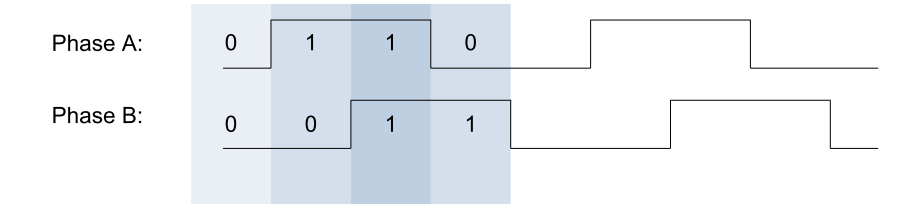
\includegraphics[scale=0.4]{Sensor/quadrature_overview.PNG}
 \end{figure}
\end{frame}

\begin{frame}{Sensorik}{Inkrementalgeber}	
 \begin{itemize}
 \item Mögliche Implementierungsstrategien
 \begin{itemize}
 \item POSIF + CCU
 \item Zwei CCU Slices
 \end{itemize}
 \end{itemize}
\end{frame}


\subsection{Temperatursensor}

\begin{frame}{Sensorik}{Temperatursensor}	
 \begin{itemize}
 \item NTC Widerstand
 \begin{itemize}
 \item Sinkender Widerstand bei steigender Temperatur
 \end{itemize}
 \item Temperaturermittlung durch Datenblatt
 \item Widerstand nicht direkt messbar
 \begin{itemize}
 \item Messung durch Spannungsteiler
 \end{itemize}
 \end{itemize}
 \begin{figure} [htbp]
 \centering
 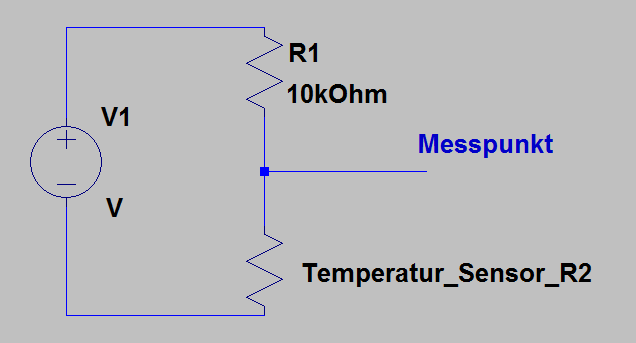
\includegraphics[scale=0.3]{Sensor/temperature_circuit.PNG}
 \end{figure}
\end{frame}

\begin{frame}{Sensorik}{Temperatursensor}	
Berechnung des Widerstands
\begin{equation}
U_{2} = \frac{U_{ges}}{R_{1} + R_{2}} * R_{2}
\end{equation}
Umstellen auf R2 durch Äquivalenzumformung
\begin{equation}
R_{2} = \frac{U_{2} * R_{1}}{U_{ges} - U_{2}}
\end{equation} 
\end{frame}

\subsection{Ausblick}
\begin{frame}{Sensorik}{Ausblick}	
 \begin{itemize}
 \item Portierung auf anderen Controller
 \item Nutzung des Inkrementalsgebers als Basis für die Kommutierung
 \end{itemize}
\end{frame}
\section{Kommunikation}
\subsection{Anforderungen}
\begin{frame}{Kommunikation}{Anforderungen}
  \begin{itemize}
    \item Controller -> PC
    \begin{itemize}
    \item Sensordaten
    \item Wiederholt
    \item Erweiterbarkeit
    \end{itemize}
    \item PC -> Controller
    \begin{itemize}
      \item Regelungsparameter
      \item Sporadisch
    \end{itemize}
  \end{itemize}
\end{frame}
\subsection{Entwurf}
\begin{frame}{Kommunikation}{Entwurf}
  \begin{itemize}
    \item Physical Layer
    \begin{itemize}
      \item UART-Baustein des $\mu$-Controllsers via USB
      \item DAVE APP zur Parametrierung
    \end{itemize}
    \item Data Link Layer
    \begin{itemize}
      \item Eigens definiertes Frame-Format
    \end{itemize}
  \end{itemize}
  \begin{center}
    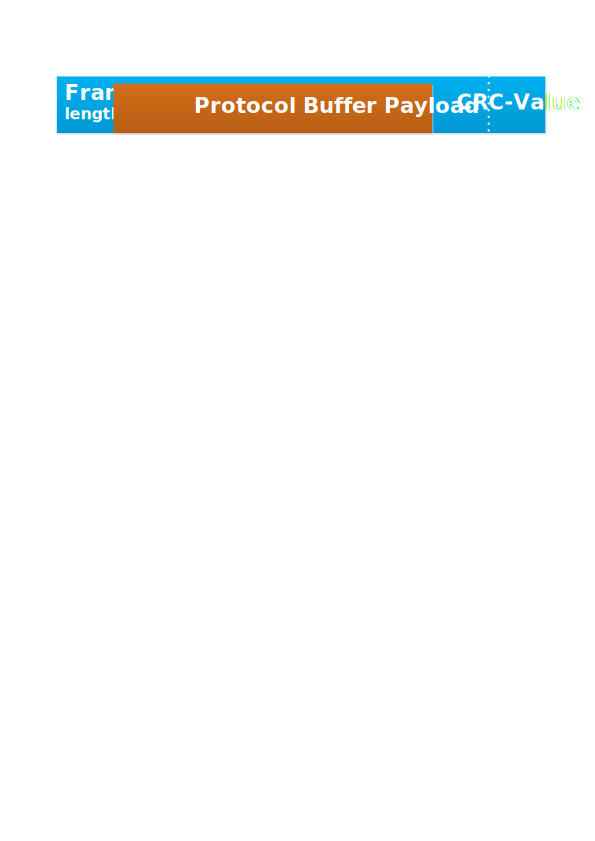
\includegraphics[width=\textwidth]{../communication/MessageFormat}
  \end{center}
\end{frame}
\begin{frame}{Kommunikation}{Entwurf}
  \begin{itemize}
    \item Restliche Layer
    \begin{itemize}
    \item Keine Adressierung, da genau zwei Teilnehmer
    \item Keine Sessions
    \item Keine Flusskontrolle
    \end{itemize}
    \item Payload: Protocol Buffer Nachricht
    \begin{itemize}
      \item Flexibilität und Erweiterbarkeit
      \item Performance
    \end{itemize}
  \end{itemize}
\end{frame}
\begin{frame}[fragile]{Kommunikation}{Entwurf}
  \begin{columns}[T]
  \begin{column}{5cm}
    \begin{itemize}
      \item Sensordaten
    \end{itemize}
    \begin{lstlisting}
    //defining an entry of the data table
    message DataEntry{
	    uint32 SensorId = 1;
	    double Data = 2;
    }
    //defining the real message
    message SensorMsg{
	    //Upcounting Nr
	    uint64 SequenceNr = 1;
	    //all Data
	    repeated DataEntry DataTable = 2;
    }
    \end{lstlisting}
  \end{column}
  \begin{column}{5cm}
    \begin{itemize}
      \item Parameter
    \end{itemize}
    \begin{lstlisting}
    //defining the parameter message
    message RegParams{
	    uint32 target = 1;
	    float paraP = 2;
	    float paraI = 3;
	    float paraD = 4;
	    float tgtVal = 5;
    }
    \end{lstlisting}
  \end{column}
  \end{columns}
\end{frame}
\subsection{Implementierung}
\begin{frame}{Kommunikation}{Implementierung}
  \begin{itemize}
    \item Frameaufbau f\"ur Sensordaten erweitert
  \end{itemize}
  \centering{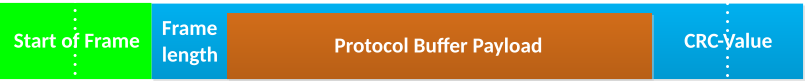
\includegraphics[width=\textwidth]{../communication/MessageFormat_enhanced}}
  \begin{itemize}
    \item PC: C\#-Bibliothek
    \begin{itemize}
    \item SerialPort-Objekt
    \end{itemize}
    \item Controller: C-Funktionen
    \begin{itemize}
      \item DAVE APP f\"ur UART
      \item DAVE APP f\"ur CRC
    \end{itemize}
  \end{itemize}
\end{frame}

\section{Regulation \& GUI Controls}
	
	\begin{frame}{Regulation \& GUI Controls}{Regulation}
	  \begin{itemize}
	    \item Regeln des Motors über Sensor und Zielwerte
	    \item GUI - Custom Controls
	  \end{itemize}
	\end{frame}

	\begin{frame}{Regulation \& GUI Controls}{Regulation - PID Regler}
			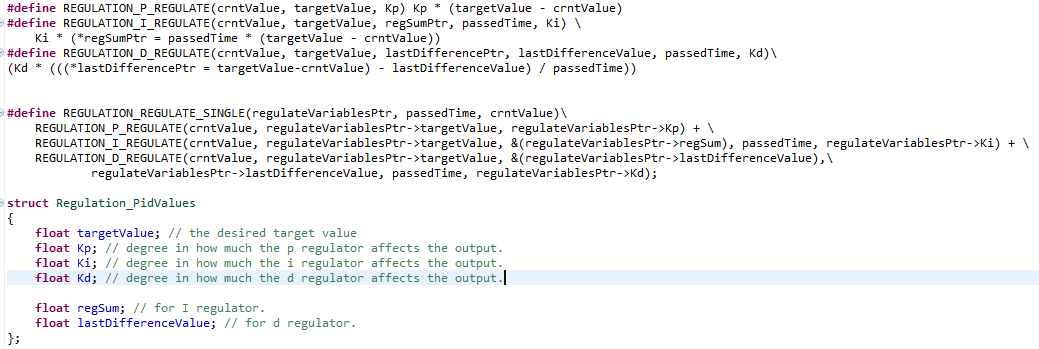
\includegraphics[width=1.05\textwidth]{../regulation/PIDRegler.png}
	\end{frame}


	\begin{frame}{Regulation \& GUI Controls}{Regulation - Main loop}
		\begin{center}			
			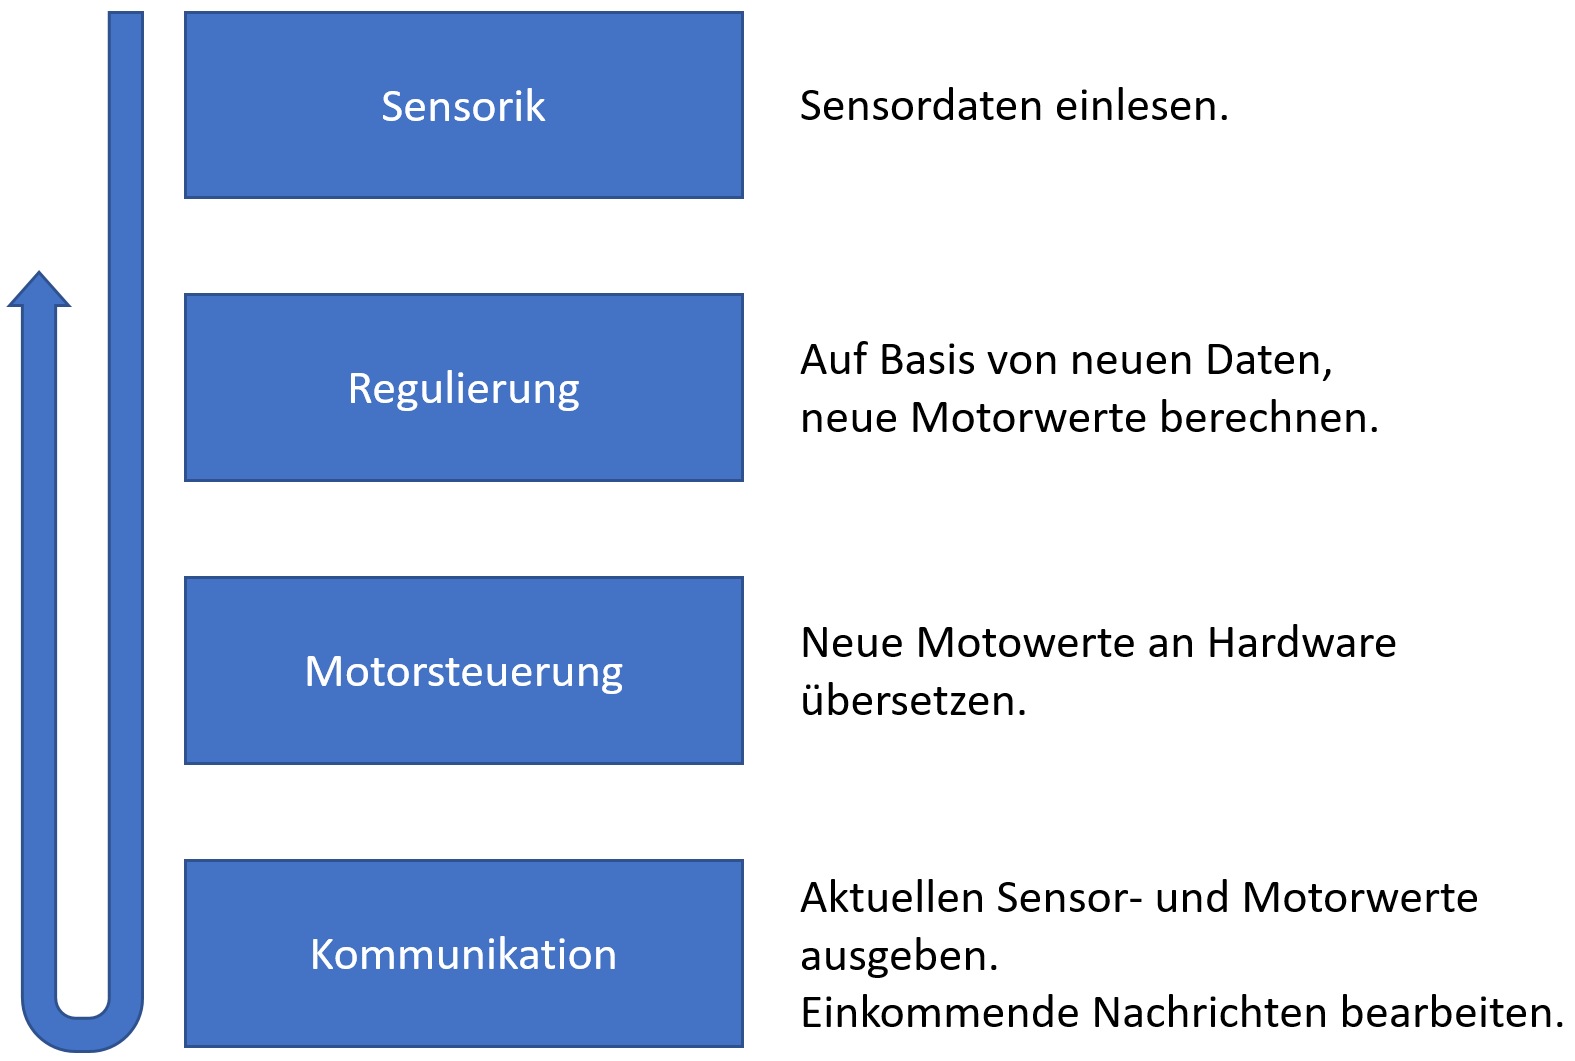
\includegraphics[width=0.9\textwidth]{../regulation/MainLoop.png}
		\end{center}
	\end{frame}


	\begin{frame}{Regulation \& GUI Controls}{Gauge Control}
		\begin{center}		
			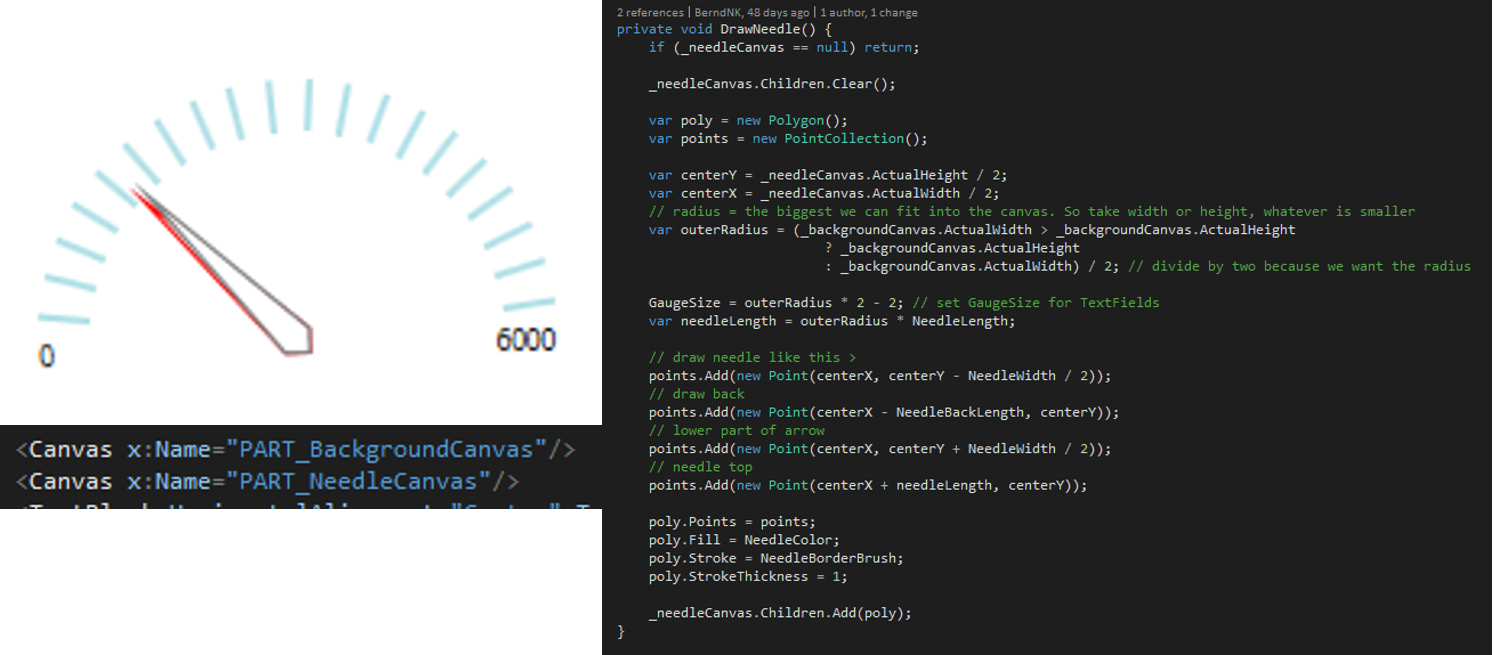
\includegraphics[width=1.05\textwidth]{../regulation/GaugeControlComplete.png}	
		\end{center}
	\end{frame}

\begin{frame}{Regulation \& GUI Controls}{Gauge Control}
	\begin{center}		
		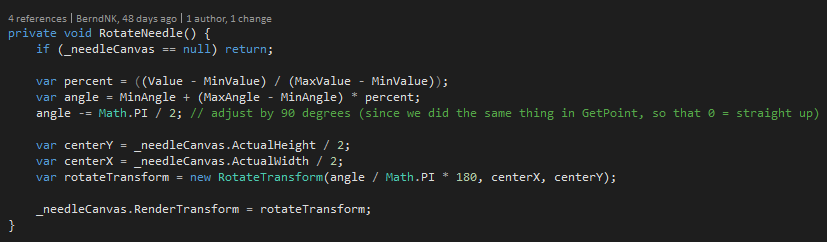
\includegraphics[width=0.9\textwidth]{../regulation/RotateNeedle.png}	
	\end{center}
\end{frame}

	\begin{frame}{Regulation \& GUI Controls}{LineChart Control}
		\begin{center}			
			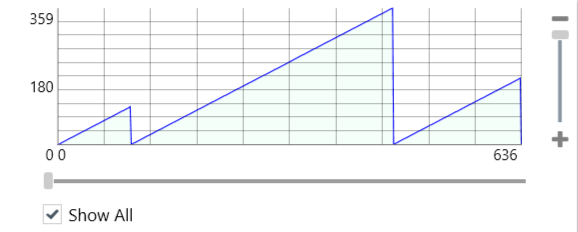
\includegraphics[width=1.05\textwidth]{../regulation/LineChart.png}
		\end{center}
	\end{frame}

	\begin{frame}{Regulation \& GUI Controls}{LineChart Control - Mehr Pixel als Sample 1}
	  	\begin{center}			
	  		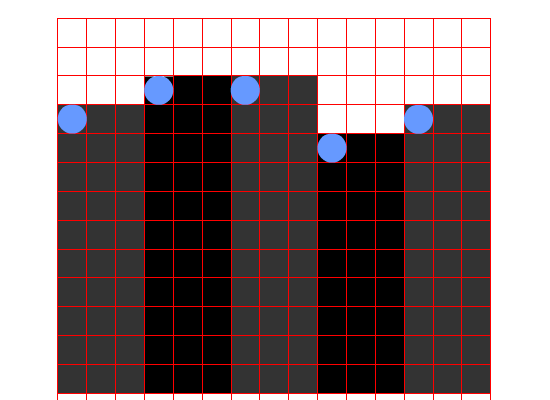
\includegraphics[width=1.05\textwidth]{../regulation/TooFewSamples01.png}
	  	\end{center}
	\end{frame}

	\begin{frame}{Regulation \& GUI Controls}{LineChart Control - Mehr Pixel als Sample 2}
	\begin{center}			
		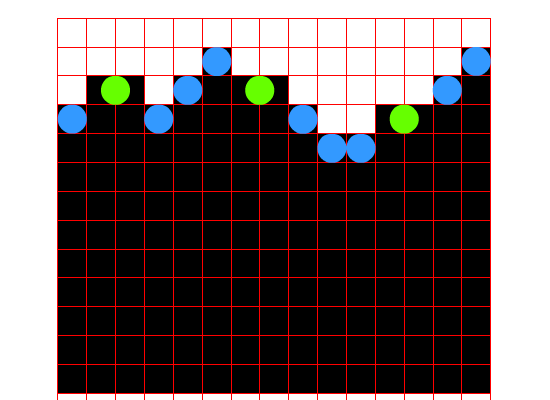
\includegraphics[width=1.05\textwidth]{../regulation/TooFewSamples02.png}
	\end{center}
	\end{frame}

	\begin{frame}{Regulation \& GUI Controls}{LineChart Control}
	\begin{center}			
		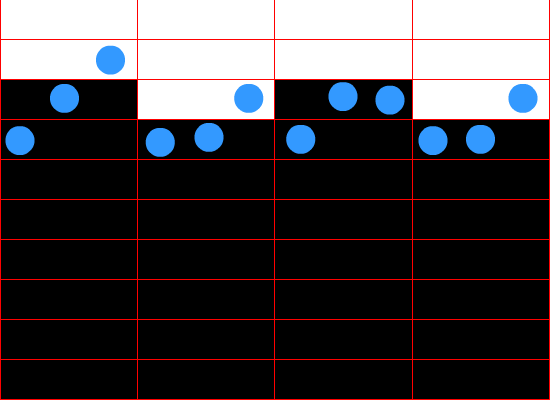
\includegraphics[width=0.8\textwidth]{../regulation/TooManySamples01.png}
	\end{center}
	\end{frame}

	\begin{frame}{Regulation \& GUI Controls}{LineChart Control}
	\begin{center}			
		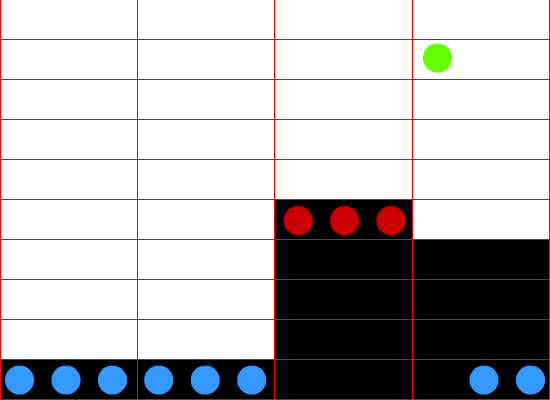
\includegraphics[width=0.8\textwidth]{../regulation/TooManySamples020001.png}
	\end{center}
	\end{frame}
	
	\begin{frame}{Regulation \& GUI Controls}{LineChart Control}
	\begin{center}			
		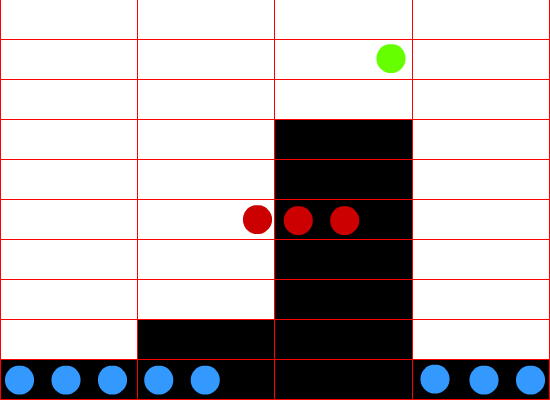
\includegraphics[width=0.8\textwidth]{../regulation/TooManySamples020002.png}
	\end{center}
	\end{frame}
	
	\begin{frame}{Regulation \& GUI Controls}{LineChart Control}
	\begin{center}			
		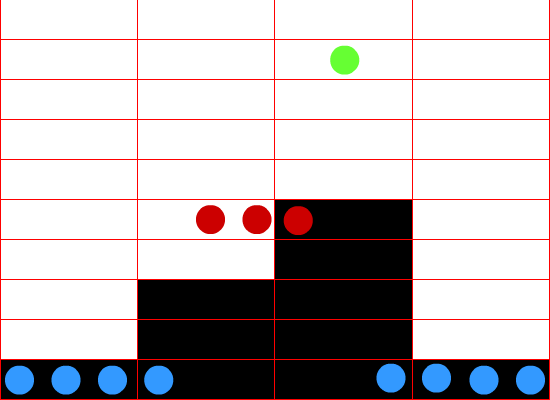
\includegraphics[width=0.8\textwidth]{../regulation/TooManySamples020003.png}
	\end{center}
	\end{frame}
	
	\begin{frame}{Regulation \& GUI Controls}{LineChart Control}
	\begin{center}			
		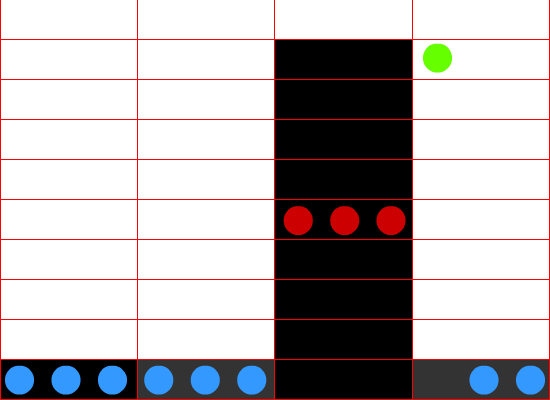
\includegraphics[width=0.8\textwidth]{../regulation/TooManySamples030001.png}
	\end{center}
	\end{frame}
	
	\begin{frame}{Regulation \& GUI Controls}{LineChart Control}
	\begin{center}			
		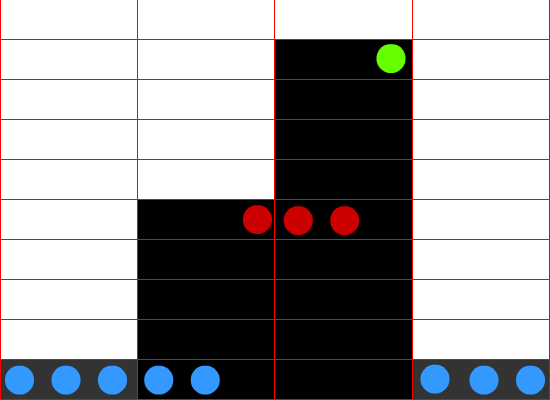
\includegraphics[width=0.8\textwidth]{../regulation/TooManySamples030002.png}
	\end{center}
	\end{frame}
	
	\begin{frame}{Regulation \& GUI Controls}{LineChart Control}
	\begin{center}			
		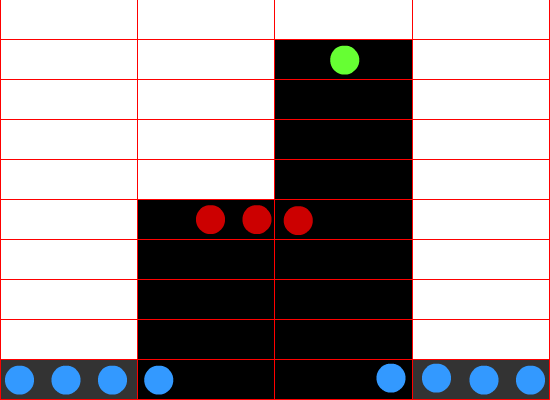
\includegraphics[width=0.8\textwidth]{../regulation/TooManySamples030003.png}
	\end{center}
	\end{frame}
	
	\begin{frame}{Regulation \& GUI Controls}{LineChart Control}
	\begin{center}			
		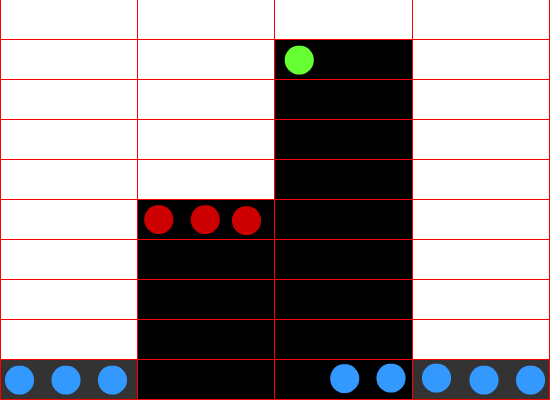
\includegraphics[width=0.8\textwidth]{../regulation/TooManySamples030004.png}
	\end{center}
	\end{frame}
	
	\begin{frame}{Regulation \& GUI Controls}{LineChart Control}
	\begin{center}			
		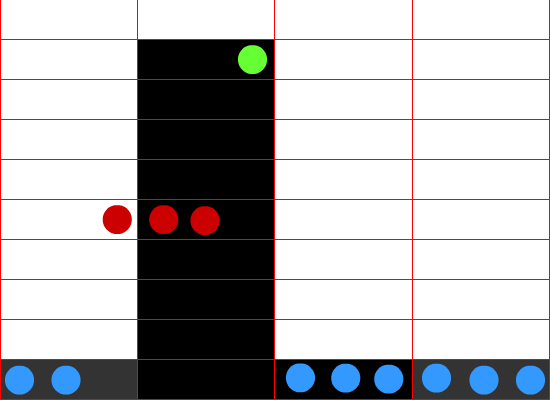
\includegraphics[width=0.8\textwidth]{../regulation/TooManySamples030005.png}
	\end{center}
	\end{frame}


	\begin{frame}{Regulation \& GUI Controls}{Plakat}
		\begin{center}			
			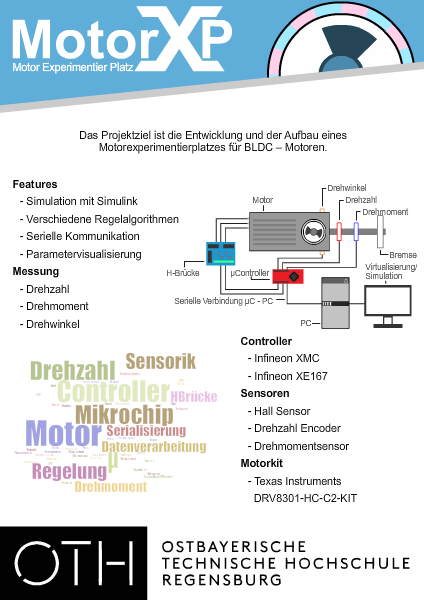
\includegraphics[height=0.6\textwidth]{../regulation/Plakat.png}
		\end{center}
	\end{frame}
\section{MotrXP GUI}

		\begin{frame}{MotrXP GUI}{Anforderungen}
		\textbf{Funktionale Anforderungen:}
	  		\begin{itemize}
	   	 		\item Anzeige der Sensordaten
	    		\item Regelung der Drehgeschwindigkeit
	    		\item Einstellung des PID Reglers
	  		\end{itemize}
	  		\textbf{Nicht-Funktionale Anforderungen:}
	  		\begin{itemize}
	   	 		\item Modulares erweiterbares System 
	    		\item Modernes Metro Design
	  		\end{itemize}
		\end{frame}

		\begin{frame}{MotrXP GUI}{Entwurf}
		\begin{minipage}{0.6\textwidth}
			\begin{itemize}
				\item Drei Schichten Architektur
	   	 		\item Entwurfsmuster
	    		\item DatenStrukturen
	    		\item Mockup
	  		\end{itemize}
		\end{minipage}
		\hfill
	  		\begin{minipage}{0.3\textwidth}
	  			\begin{figure}[htbp]
	  				\centering
	  				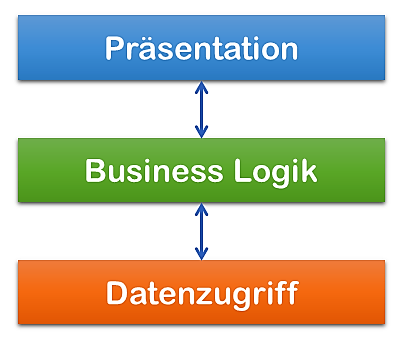
\includegraphics[width=\textwidth]{../gui/Bilder/Arc1.png}
	  			\end{figure}
	  			\begin{figure}[h]
	  				\centering
	  				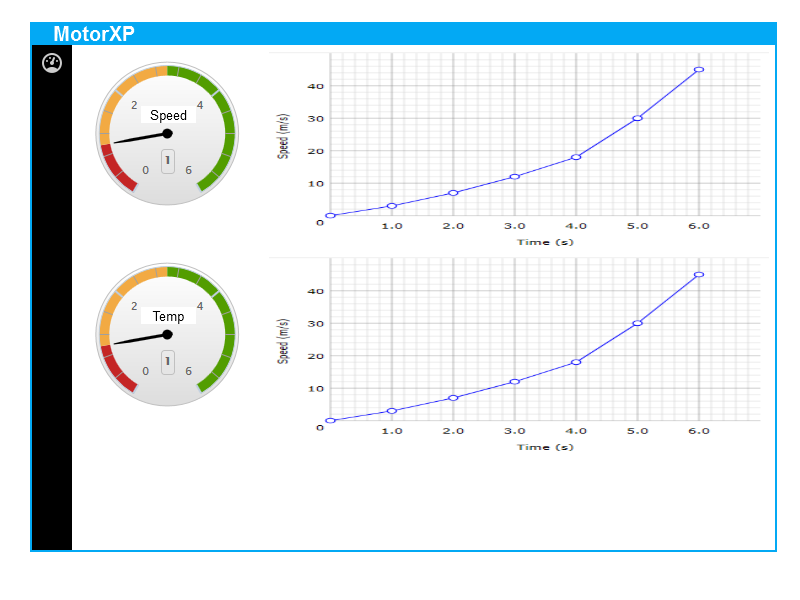
\includegraphics[width=\textwidth]{../gui/Bilder/Mockup.png}
	  			\end{figure}
	  		\end{minipage}
	  		
	  		
		\end{frame}

		\begin{frame}{MotrXP GUI}{Implementierung}
		\begin{minipage}{0.5\textwidth}
			\begin{itemize}
				\item MVVM-Light Framework
				\item MahApps Metro UI Toolkit
				\item Custom Controls 
			\end{itemize}
		\end{minipage}
		\hfill
		\begin{minipage}{0.4\textwidth}
			\begin{figure}[h]
	  			\centering
	  				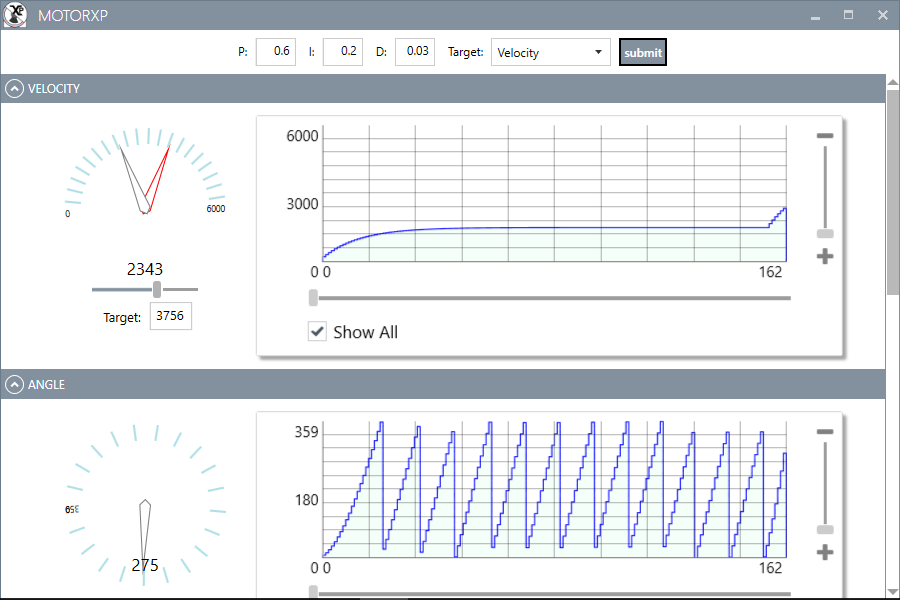
\includegraphics[width=\textwidth]{../gui/Bilder/GUIScreenshot2.png}
	  		\end{figure}
		\end{minipage}
	  		
		\end{frame}


		\begin{frame}{MotrXP GUI}{Ausblick}
\begin{figure}
	  			\centering
	  				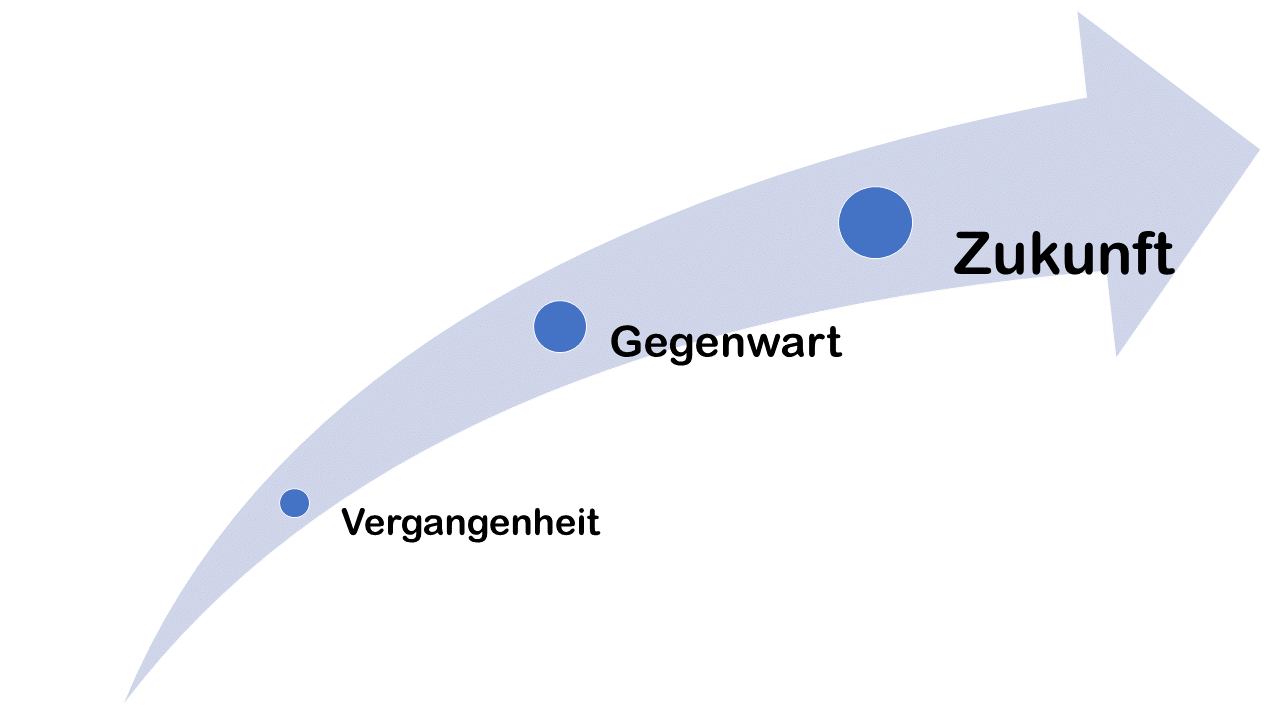
\includegraphics[width=\textwidth]{../gui/Bilder/AusblickPfeil.png}
	  		\end{figure}
		\end{frame}
\author{Christian Brunner}
\section{Test und Analyse}

\begin{frame}{Test und Analyse}{Übersicht}
	\begin{itemize}	
		\item Spannungssignal
		\item Hall-Sensoren
		\item XMC 4700 Relax Kit
		\item Steuerung BLDC
	\end{itemize}
\end{frame}

\begin{frame}{Test und Analyse}{Spannungsmessung Fremderregung}
	\begin{figure}
		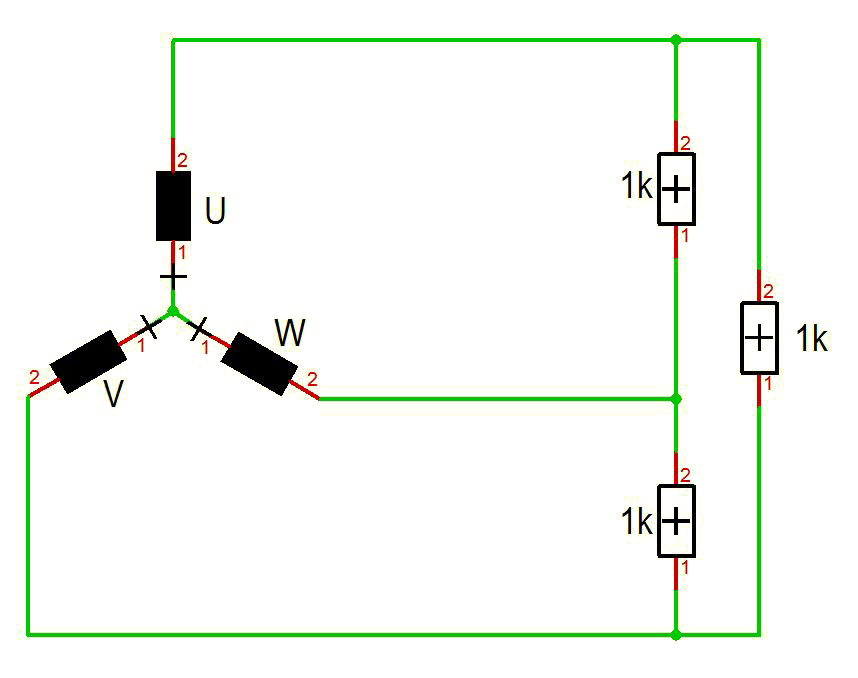
\includegraphics[height=\textheight]{Test/Messchaltung_Fremderregung}
		\caption{Messchaltung}
	\end{figure}
\end{frame}

\begin{frame}{Test und Analyse}{Analyse Spannungsmessung Fremderregung}
	\begin{figure}
		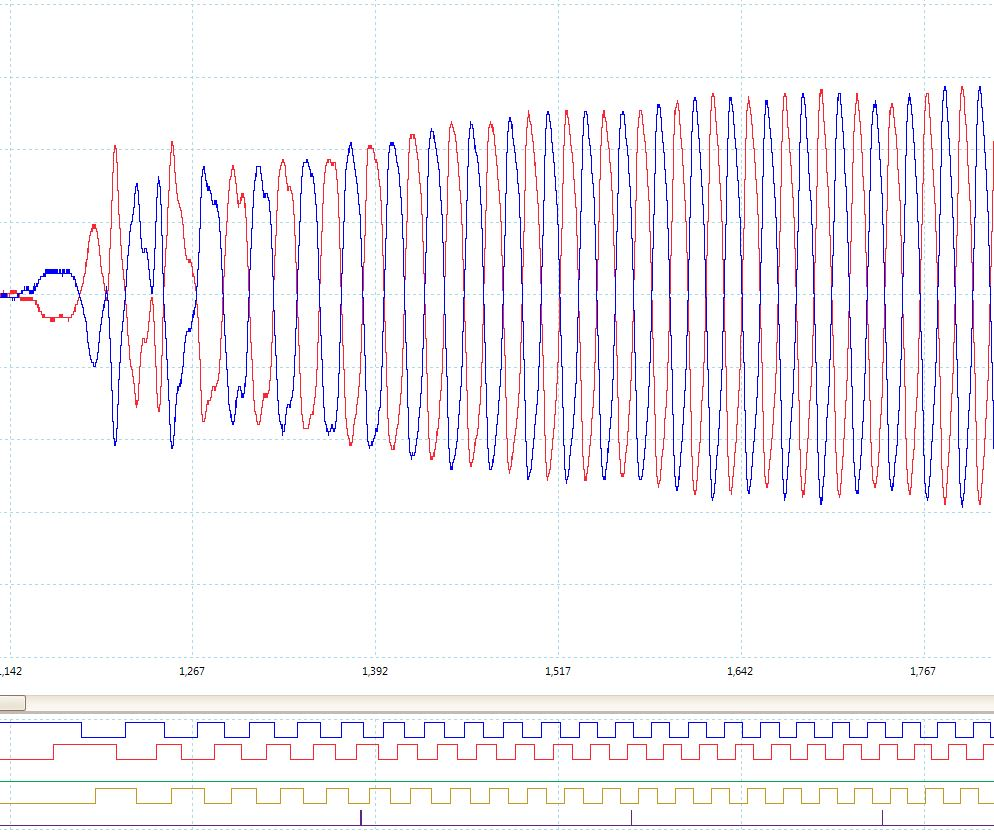
\includegraphics[height=\textheight]{Test/Spannungssignal_Messung}
	\end{figure}
\end{frame}

\begin{frame}{Test und Analyse}{Analyse Spannungsmessung Fremderregung mit Störsignalen}
	\begin{figure}
		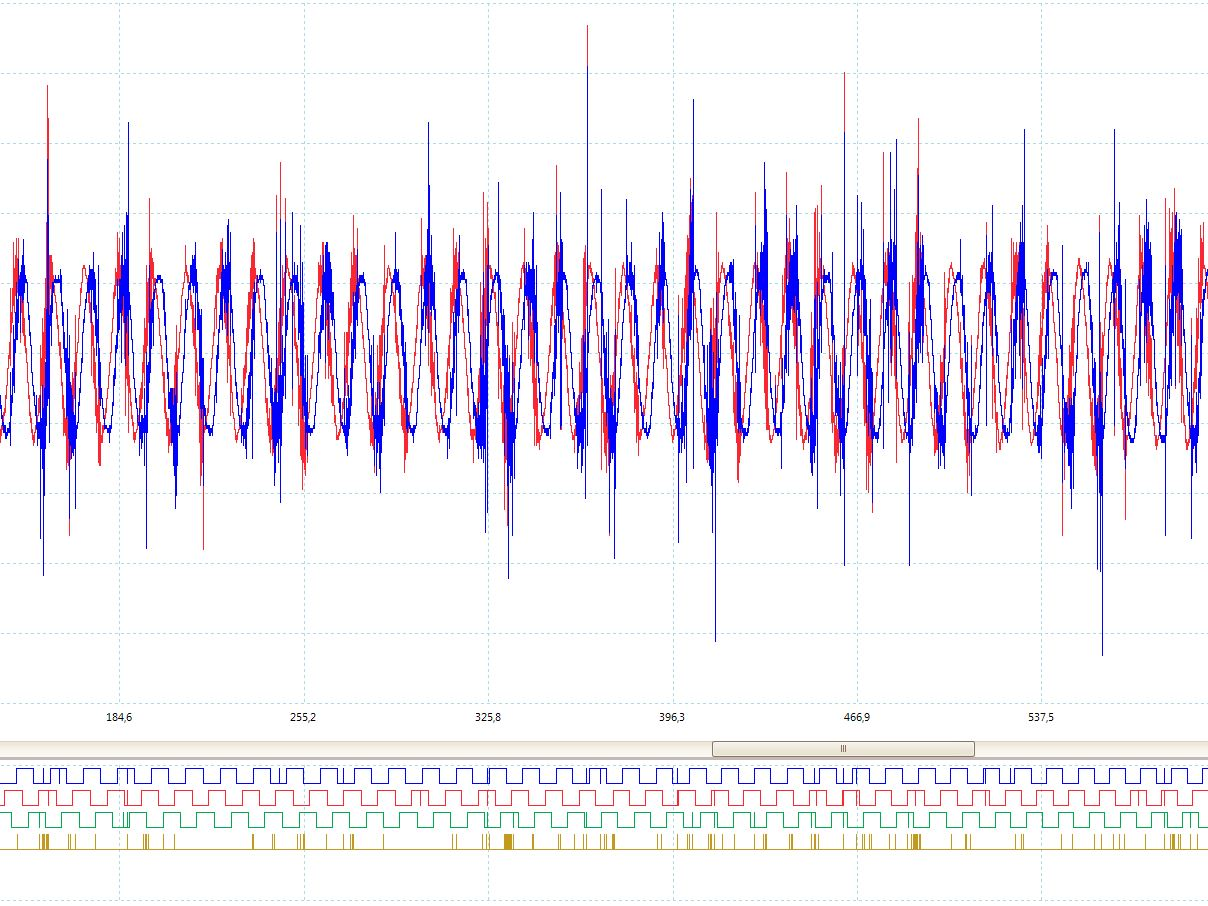
\includegraphics[width=\textwidth]{Test/Spannungssignal_Messung_mit_Fehler}
	\end{figure}
\end{frame}

\begin{frame}{Test und Analyse}{Hall-Sensoren in Verbindung mit dem XMC 4700 Relax Kit 5V}
	\begin{itemize}
		\item XMC 4700 Relax Kit 5V
		\begin{itemize}
			\item Vorbereitet für Arduino Shields (5V)
			\item Pegelwandler (5V $\leftrightarrow$ 3.3V)
			\item Störempfindlich gegenüber längeren Messleitungen ($\approx$ 20 cm)
		\end{itemize}
	\end{itemize}
\vspace{\baselineskip}
\vspace{\baselineskip}
\end{frame}

\begin{frame}{Test und Analyse}{Hall-Sensoren in Verbindung mit dem XMC 4700 Relax Kit 5V}
	\begin{figure}
		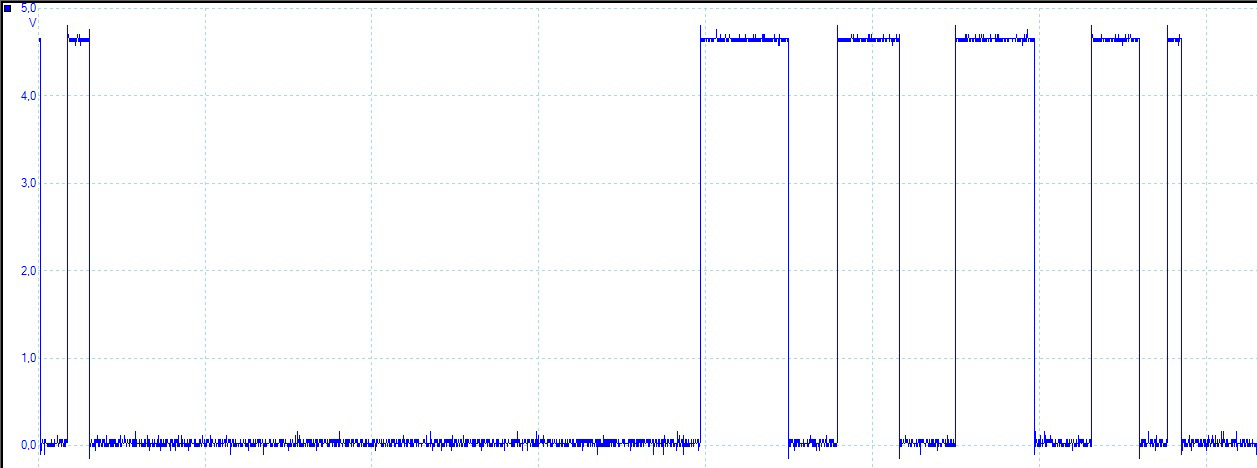
\includegraphics[height=0.4\textheight]{Test/hall_ok}
		\vspace{\baselineskip}
		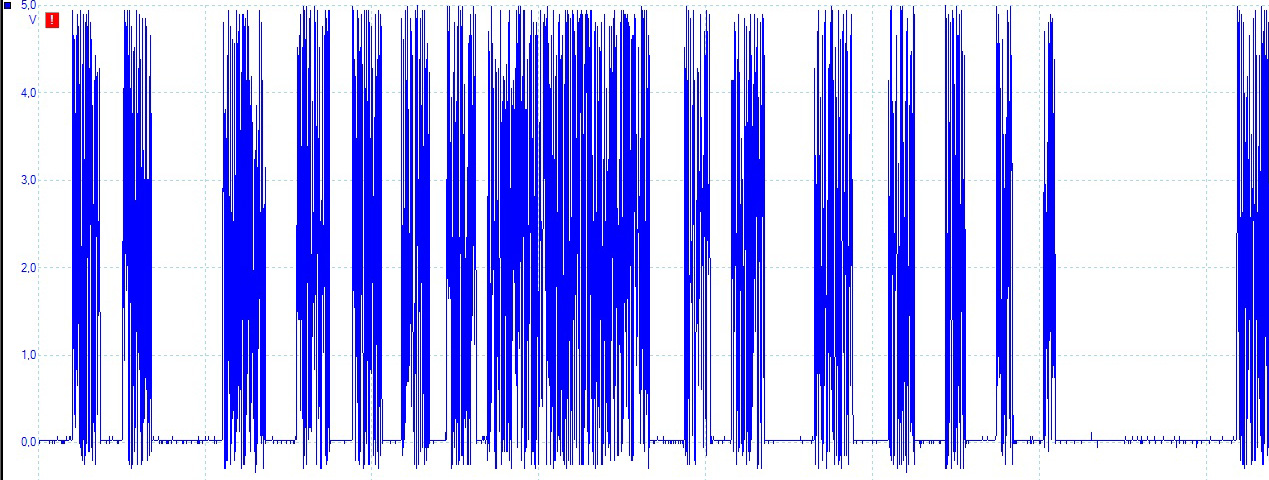
\includegraphics[height=0.4\textheight]{Test/hall_jitter_4700}
	\end{figure}
\end{frame}


\begin{frame}{Test und Analyse}{Hall-Sensoren in Verbindung mit dem XMC 4700 Relax Kit 5V}
	\begin{itemize}
		\item XMC 4700 Relax Kit 5V
		\begin{itemize}
			\item Vorbereitet für Arduino Shields (5V)
			\item Pegelwandler (5V $\leftrightarrow$ 3.3V)
			\item Störempfindlich gegenüber längeren Messleitungen ($\approx$ 20 cm)
		\end{itemize}
		\item $\rightarrow$ Messleitung verkürzen
		\item $\rightarrow$ Pegelwandler austauschen/entfernen
	\end{itemize}
\end{frame}

\begin{frame}{Test und Analyse}{Steuerung BLDC - Schaltung}
	\begin{figure}
		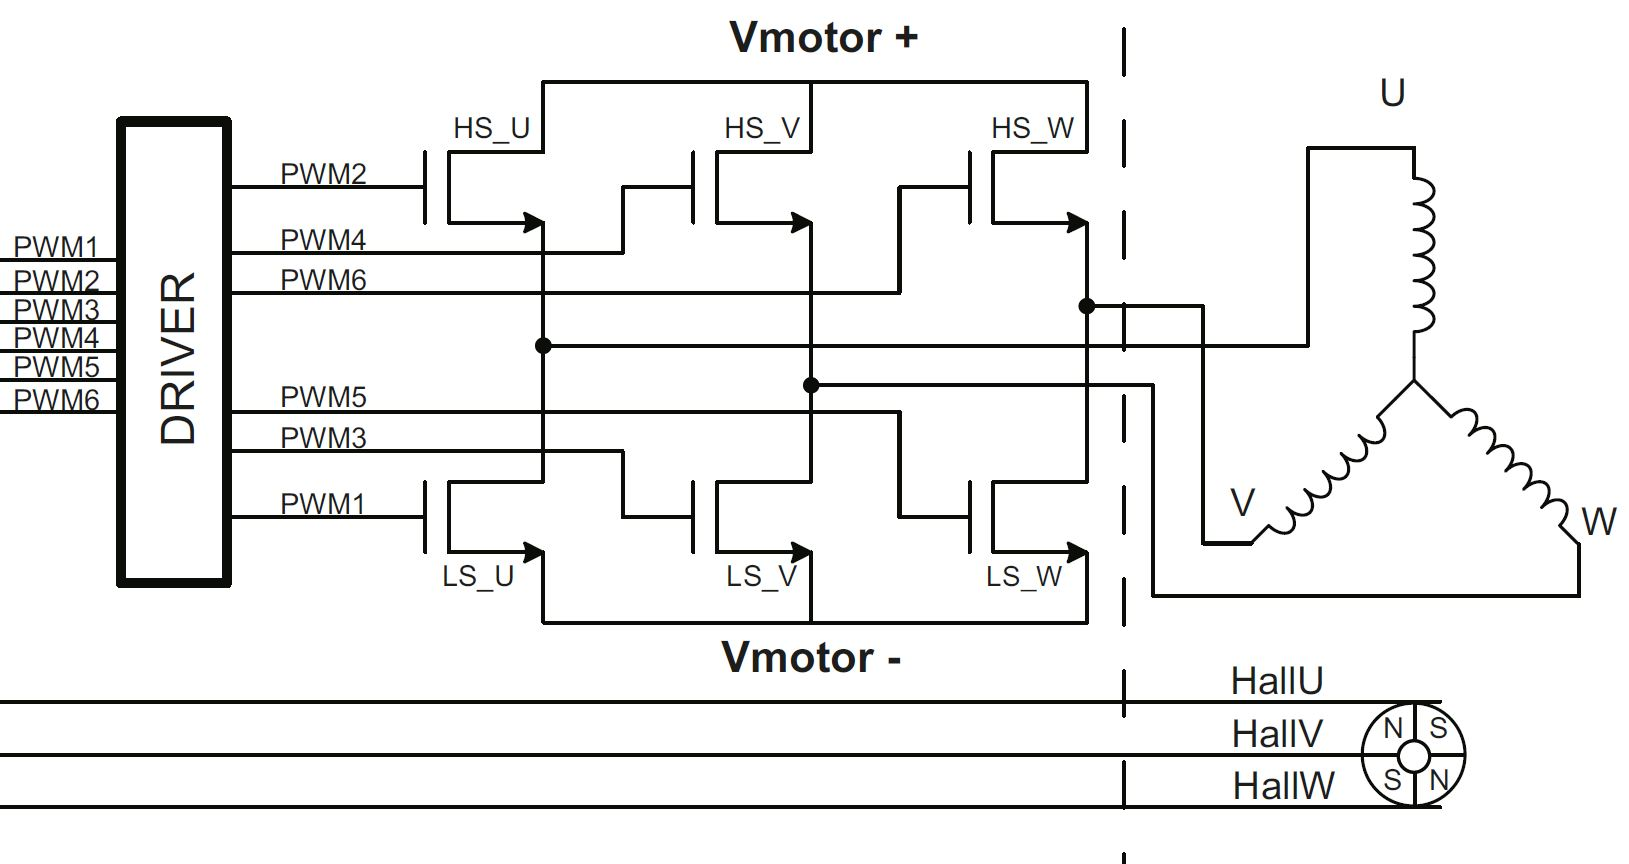
\includegraphics[width=\textwidth]{Test/Aufbau_Ansteuerung_Motor}
	\end{figure}
\end{frame}

\begin{frame}{Test und Analyse}{Steuerung BLDC - Steuersignal}
	\begin{figure}
		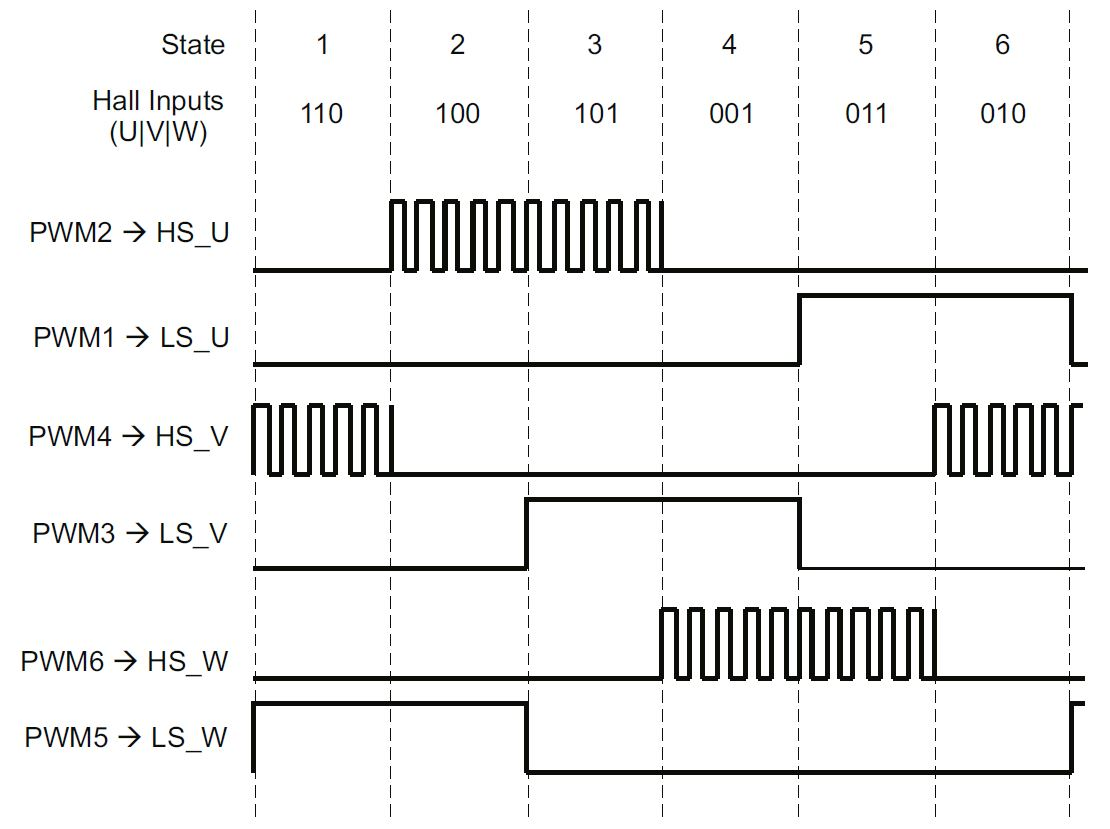
\includegraphics[height=0.8\textheight]{Test/Ansteuerung_H-Bruecke}
	\end{figure}
\end{frame}

\begin{frame}{Test und Analyse}{Steuerung BLDC - Texas Instrument}
	\begin{figure}
		\begin{itemize}
			\item Abweichende Signale
			\item Zwei Ausgänge gleichzeitig HIGH
		\end{itemize}
		\vspace{\baselineskip}
		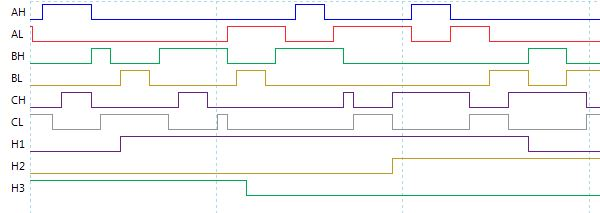
\includegraphics[width=\textwidth]{Test/Steuersignale_TI}
	\end{figure}
\end{frame}

\section{Simulation}
	
	\subsection{Anforderungen I}
	\begin{frame}{Simulation}{Anforderungen}
	  \begin{itemize}
	    \item Kommunikation mit GUI
	    \item Simulation in Echtzeit
	    \item Kommunikation mittels serieller Schnittstelle
	  \end{itemize}
	\end{frame}

	\subsection{Entwurf I}
	\begin{frame}{Simulation}{Entwurfsphase und Implementierung I}
	  	\begin{figure}[htbp]
	  		\centering
	  		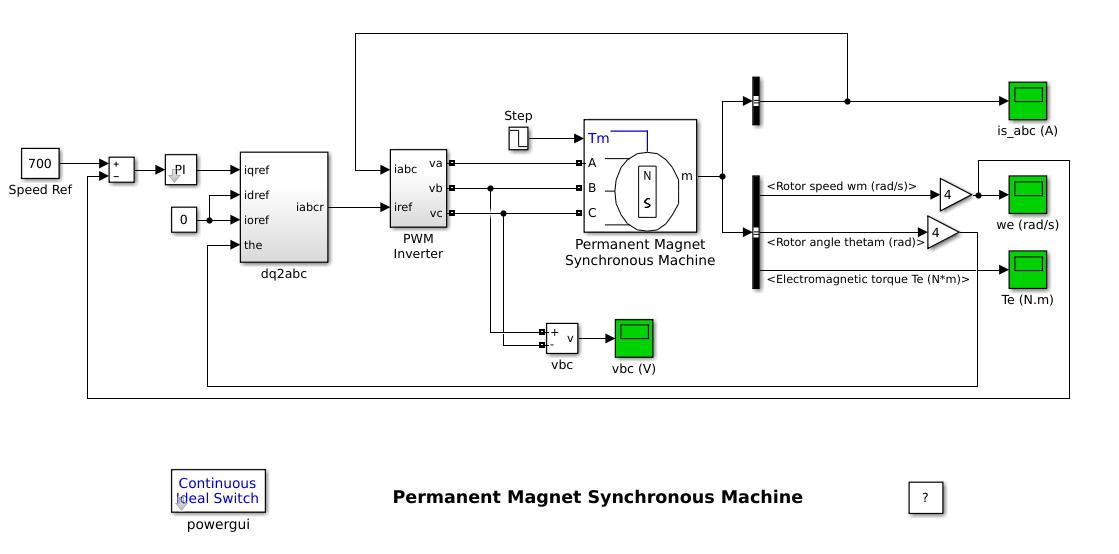
\includegraphics[width=\textwidth]{../sim/pictures/powerPmmotor.png}
	  	\end{figure}
	\end{frame}

	\subsection{Analysephase II}
	\begin{frame}{Simulation}{Analysephase II}
		\begin{center}
		\begin{tabular}{cc}
			\begin{minipage}{0.4\textwidth} 
				\includestandalone[width=\textwidth]{../sim/pictures/motorAufbau}
			\end{minipage}	
			&  
			\begin{minipage}{0.4\textwidth}
				\vspace{-0.35cm}
				\includestandalone[width=0.9\textwidth]{../sim/pictures/vereinfachtesModell}	
			\end{minipage}	
			\\ 
		\end{tabular} 
	
		\vspace{0.5cm}
		\includestandalone[width=0.8\textwidth]{../sim/pictures/abgerolltesModell}
	\end{center}
	\end{frame}

	\subsection{Bewertung des neuen Modells}
	\begin{frame}{Simulation}{Bewertung}
		\begin{itemize}
			\item Resultierendes Spulenfeld
				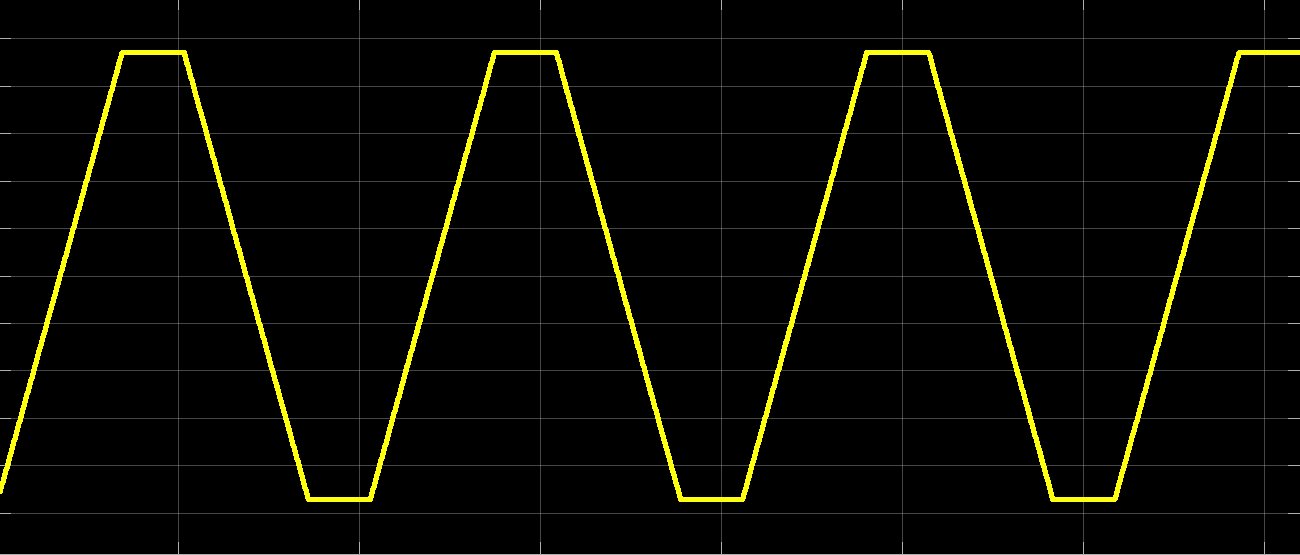
\includegraphics[width=0.8\textwidth]{../sim/pictures/resultierendesFeld.png}
				\newline
				$\sum \limits_1^{28} V_{res_i} = \sum \limits_1^{28} (V_i+R_i) = \sum \limits_1^{28} V_i + \sum \limits_1^{28} R_i$
		\end{itemize}	 
	\end{frame}

	\begin{frame}{Simulation}{Bewertung}
		\begin{itemize}
			\item Drehmoment
			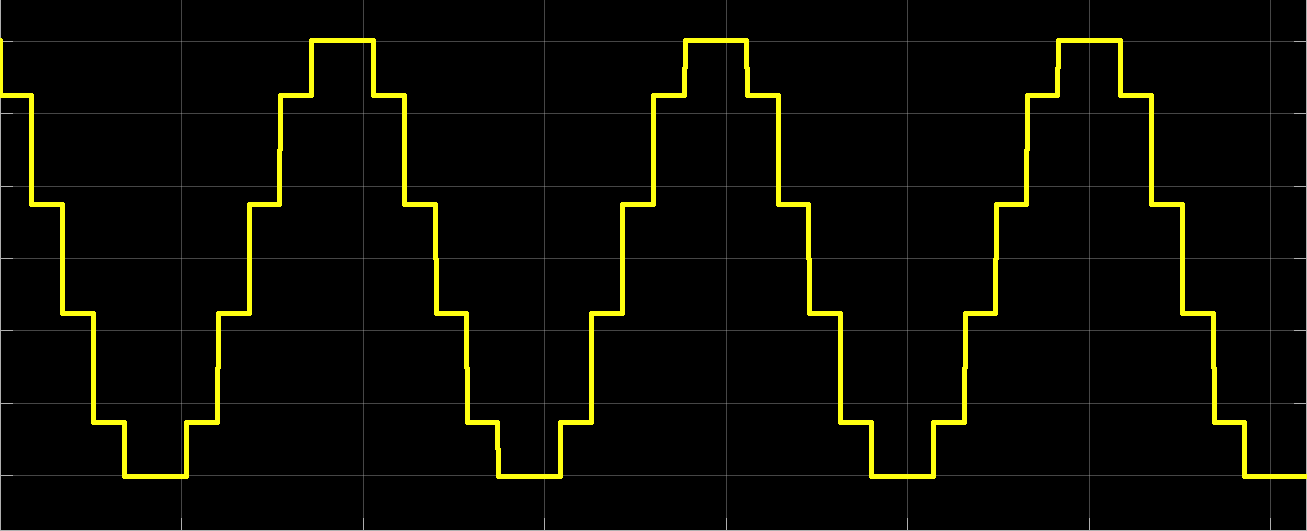
\includegraphics[width=0.8\textwidth]{../sim/pictures/drehmoment.png}
		\end{itemize}
	
	\end{frame}

\begin{frame}{Abschluss}
\centering 
	\begin{huge}
		\textbf{Vielen Dank}
	\end{huge}
\end{frame}


\end{document}
